\documentclass[11pt]{article}
\usepackage{amnat}

\title{Supplementary text and figures}
\date{\vspace{-5ex}}

\begin{document}

\maketitle

Supplementary text and figures for sensitivity analyses with respect to Fig.~3a and Fig.~5 from the main manuscript.

Figure S1 shows the minimum temperature for completing warm-up for different values of convection $K_2$ (Fig.~S1a--c), conductance $K_1$ (Fig.~S1d--f), and intensity of solar radiation (Fig.~S1g--i).
For convection and conductance, solid thin lines represent default values (see Table~1 in the main text).
The default values are then multiplied by 10 (thick lines) or by 0.1 (dashed lines).
The main qualitative difference is for endotherms when conductance is too high (thick line Fig.~S1f), most of the heat generated endogenously dissipates in the environment.
As a consequence, there is not much difference between small and large individuals.

Figure S2 shows the effect of relaxing constant temperature.
The horizontal axis shows temperature from sunrise (coldest), increasing linearly until mid-afternoon (midpoint between noon and sunset), and then decreasing.
The hottest temperature is defined as $10 ^{\circ}\rm{C}$ hotter than the temperature at sunrise.
Figure S2 shows that allowing for daily environmental temperature variation does not change the qualitative results (see Fig.~5 in the main text).

For all the figures, the remaining parameters are the same as in the main text.

\renewcommand{\thefigure}{S\arabic{figure}}

\begin{figure}[h]
    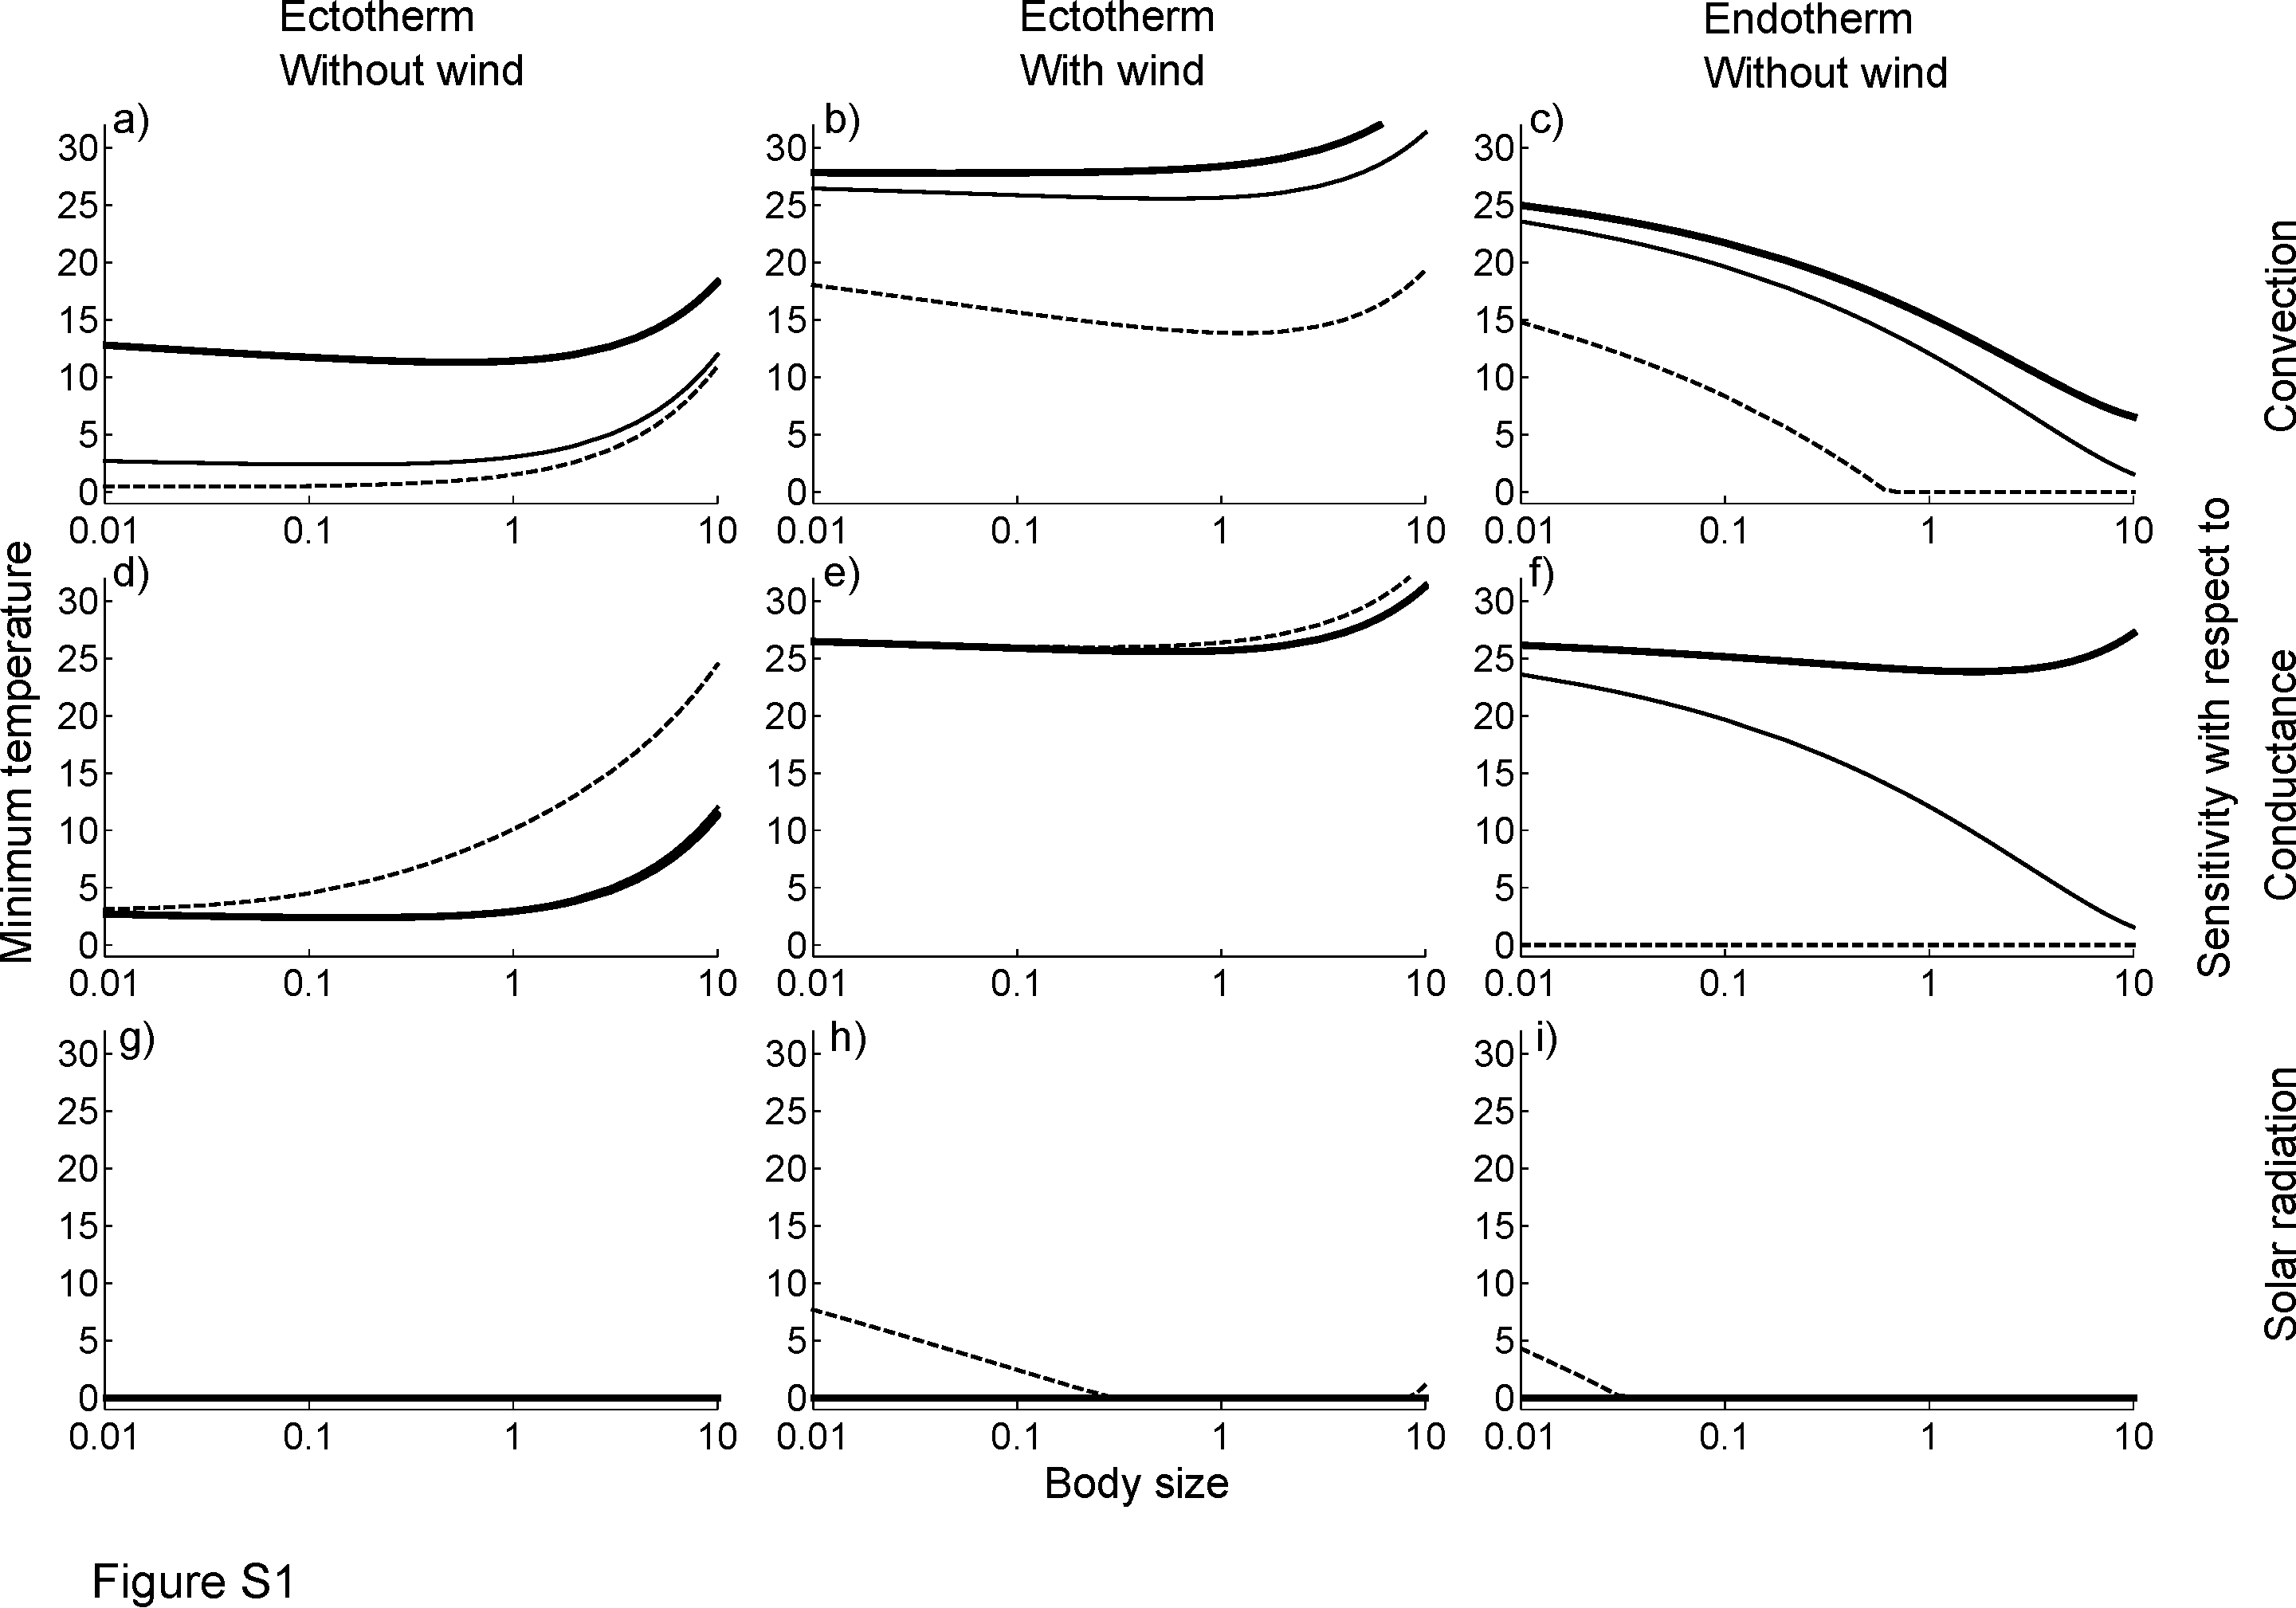
\includegraphics[width=\textwidth]{figS1}
	\caption{} % TODO
	\label{fig:S1}
\end{figure}

\begin{figure}[h]
    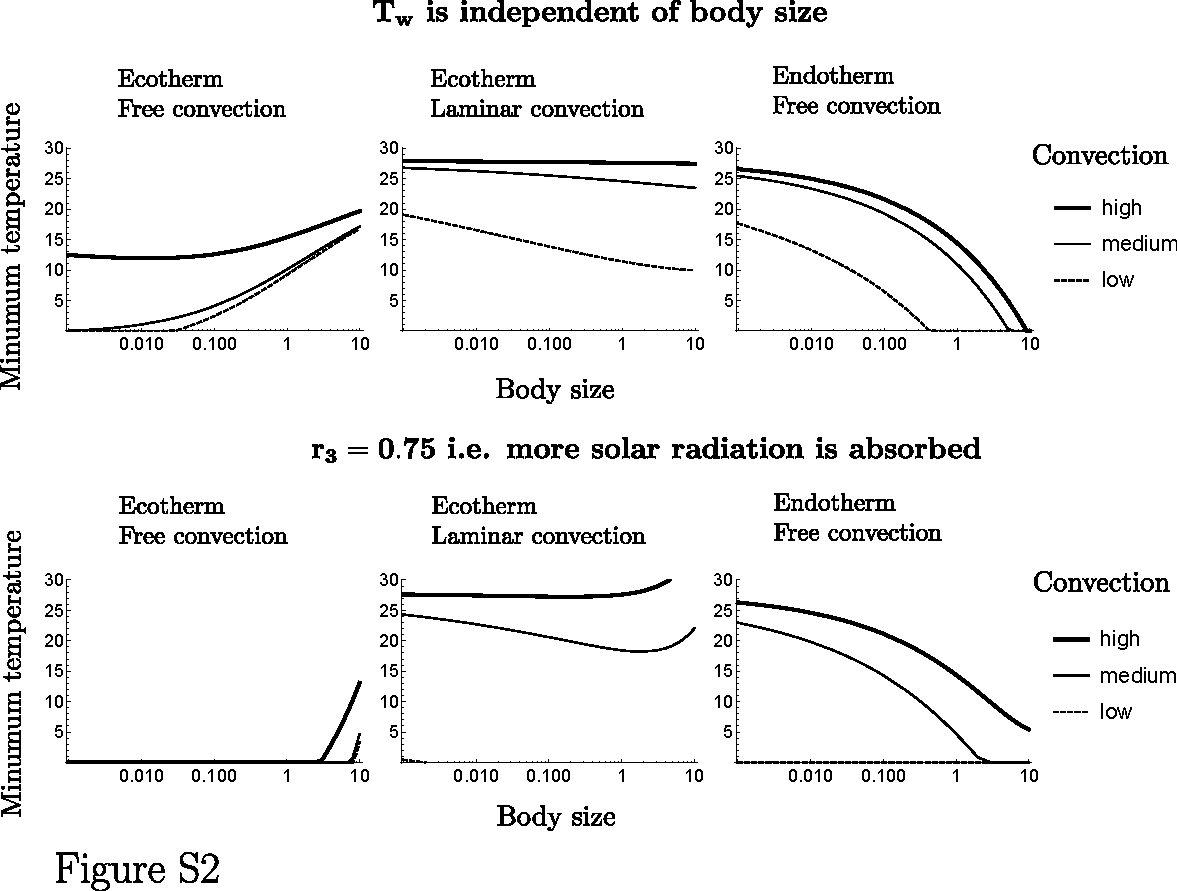
\includegraphics[width=\textwidth]{figS2}
	\caption{} % TODO
	\label{fig:S2}
\end{figure}

\end{document}
